\documentclass{beamer}
\usetheme{CambridgeUS}

\usepackage{pgfplots}
\pgfplotsset{compat=1.8}
\usepgfplotslibrary[statistics]

\author{Steven Bethard}
\title{Major Field Test}

\begin{document}

\begin{frame}
\titlepage
\end{frame}

\begin{frame}{Overall Results}
\begin{tikzpicture}
\begin{axis}[
  ybar interval,
  ylabel={Number of students},
  ytick=data,
  xlabel={Scaled score},
  xmin=145,
  xmax=175,
  xticklabel=\pgfmathprintnumber\tick--\pgfmathprintnumber\nexttick,
  width=\textwidth,
  height=0.8\textheight]
\addplot+[hist={bins=6}]
  table[row sep=\\,y index=0]
    {data\\ 147\\ 173\\ 158\\ 154\\ 146\\};
\end{axis}
\end{tikzpicture}
\end{frame}

\begin{frame}{Results by Area}
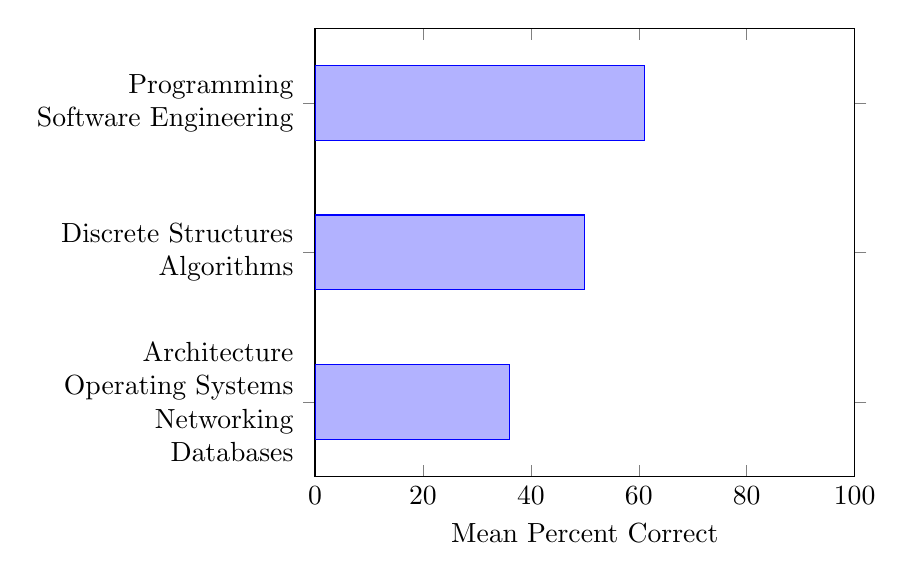
\begin{tikzpicture}
\begin{axis}[
  xbar,
  xlabel={Mean Percent Correct},
  xmin=0,
  xmax=100,
  yticklabels={
    Programming\\Software Engineering,
    Discrete Structures\\Algorithms,
    Architecture\\Operating Systems\\Networking\\Databases},
  yticklabel style={align=right},
  ytick=data,
  bar width=0.5,
  enlarge y limits=0.25]
\addplot coordinates {
  (61,3)
  (50,2)
  (36,1)};
\end{axis}
\end{tikzpicture}
\end{frame}

\end{document}